\documentclass[final]{siamart171218}
%\VignetteIndexEntry{Algorithms for NMF and topic modeling}
%\VignettePackage{fastTopics}
\usepackage{amsmath}
\usepackage{amssymb}
\usepackage{bm}
\setlength{\oddsidemargin}{0.65in}
\setlength{\evensidemargin}{0.65in}

\title{Algorithms for fitting topic models and non-negative matrix factorizations to count data}
\author{Peter Carbonetto and Matthew Stephens\thanks{Department of Human Genetics and the Research Computing Center, University of Chicago, Chicago, IL}}

\usepackage{Sweave}
\begin{document}

\maketitle

\section{Introduction}

In this example we embed parts of the examples from the
\texttt{kruskal.test} help page into a \LaTeX{} document:
\begin{Schunk}
\begin{Sinput}
> data(airquality, package = "datasets")
> library("stats")
> kruskal.test(Ozone ~ Month,data = airquality)
\end{Sinput}
\begin{Soutput}
	Kruskal-Wallis rank sum test

data:  Ozone by Month
Kruskal-Wallis chi-squared = 29, df = 4, p-value = 7e-06
\end{Soutput}
\end{Schunk}

which shows that the location parameter of the Ozone distribution
varies significantly from month to month. Finally, we include a
boxplot of the data, using
\begin{Schunk}
\begin{Sinput}
> boxplot(Ozone ~ Month, data = airquality)
\end{Sinput}
\end{Schunk}
\begin{center} 
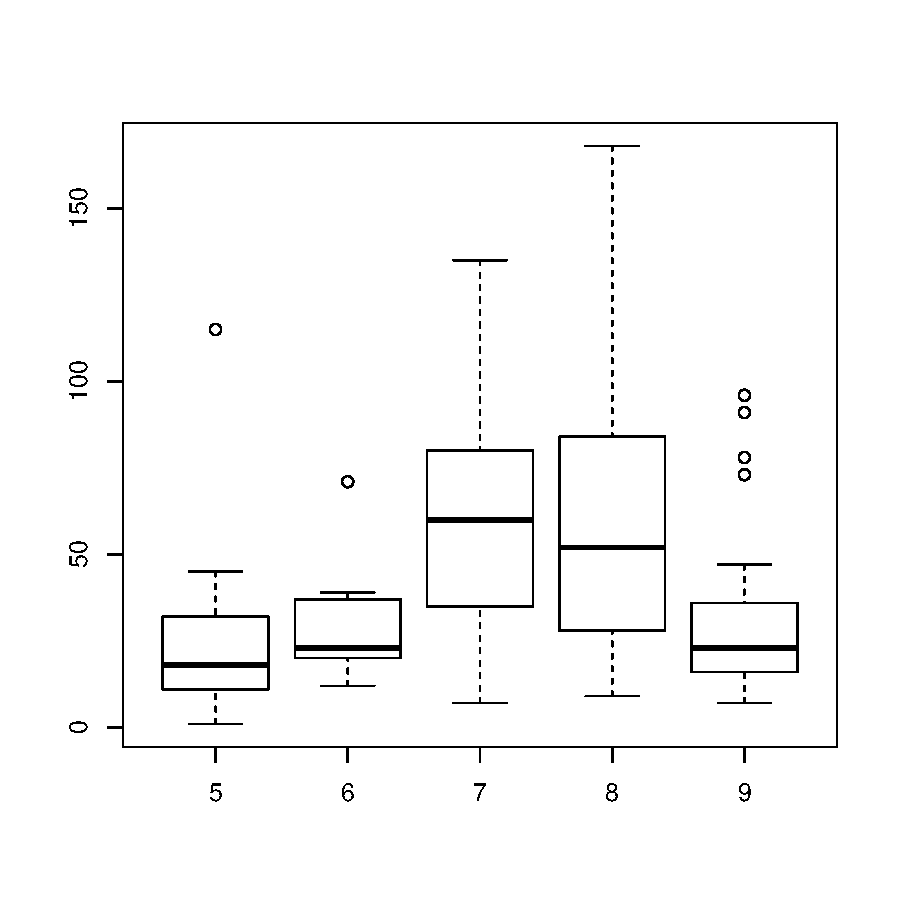
\includegraphics{algorithms-003}
\end{center}

Here is a citation: \cite{lee-2001}.

\bibliographystyle{siamplain}
\bibliography{algorithms}

\end{document}
